
\documentclass[12pt]{amsart}
\usepackage{geometry} % see geometry.pdf on how to lay out the page. There's lots.
\usepackage{graphicx}
\usepackage{natbib}
\usepackage{amsmath}
\usepackage{listings}
%\geometry{a4paper} % or letter or a5paper or ... etc
% \geometry{landscape} % rotated page geometry

% See the ``Article customise'' template for come common customisations

\title{The ModelGrid Package}
\author{Greg Tucker}
%\date{First version, May 2013} % delete this line to display the current date

%%% BEGIN DOCUMENT
\begin{document}

\lstset{ %
language=Python,                % choose language
basicstyle=\footnotesize,       % size of fonts used for code
numbers=left,                   % where to put line-numbers
numberstyle=\footnotesize,      % size used for line-numbers
stepnumber=1,                   % the step between two line-numbers. If it is 1 each line will be numbered
numbersep=5pt,                  % how far the line-numbers are from the code
%backgroundcolor=\color{white},  % choose the background color. You must add \usepackage{color}
showspaces=false,               % show spaces adding particular underscores
showstringspaces=false,         % underline spaces within strings
showtabs=false,                 % show tabs within strings adding particular underscores
frame=single,           % adds a frame around the code
tabsize=2,          % sets default tabsize to 2 spaces
captionpos=b,           % sets the caption-position to bottom
breaklines=true,        % sets automatic line breaking
breakatwhitespace=false,    % sets if automatic breaks should only happen at whitespace
columns=fullflexible,
basicstyle=\ttfamily,
escapeinside={\%*}{*)}          % if you want to add a comment within your code
}

\maketitle
%\tableofcontents

\section{Overview}

ModelGrid is an open-source software package that creates and manages a regular or irregular grid for building 2D numerical simulation models. ModelGrid is especially useful for finite-volume (FV) and finite-difference (FD) models, but also can be used for a variety of other applications. ModelGrid provides efficient built-in functions for common operations in FD and FV models, such as calculating local gradients and integrating fluxes around the perimeter of grid cells. Staggered-grid models are especially easy to implement with ModelGrid.
A novel feature of ModelGrid is the ability to switch seamlessly between structured and unstructured grids.

This document provides a basic introduction to building applications using ModelGrid. It covers: (1) how grids are represented, (2) a tutorial example in building a diffusion-model application, and (3) a guide to ModelGrid's methods and data structures. ModelGrid is written in python. It is a component of the Landlab modeling package.

\subsection{How a Grid is Represented}

%%%%%%%%%%% FIGURE %%%%%%%%%%%
 \begin{figure}[h!]
    \centering
    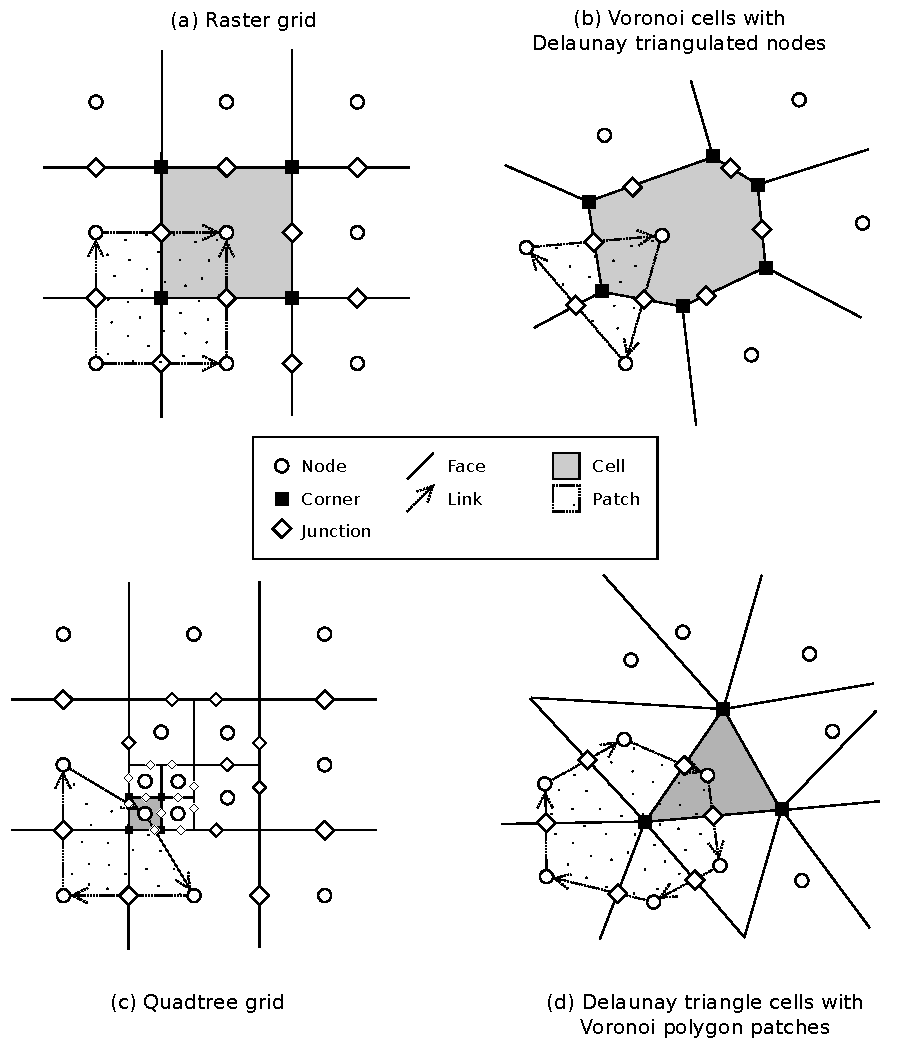
\includegraphics[scale=0.9]{grid_schematic.pdf}
    \caption{Elements of a model grid. Each grid comprises nodes, cells, faces, corners, patches, links, directed edges, and junctions. (Note that not all links, edges, and patches are shown, and only one representative cell is shaded.)}
   \label{grid}
\end{figure}
%%%%%%%%%%%%%%%%%%%%%%%%%%%

Figure~\ref{grid} illustrates how ModelGrid represents a simulation grid. The grid contains a set of $(x,y)$ points called {\em nodes}. In a typical finite-difference model, nodes are the locations at which one tracks scalar state variables, such as water depth, land elevation, or temperature. Each node is associated with a polygon called a {\em cell}. Each cell is bounded by a set of line segments known as {\em faces}, which it shares with its neighboring cells.

In the simple case of a regular (raster) grid, the cells are square, the nodes are the center points of the cells (Figure~\ref{grid}a), and the faces have identical length (equal to the node spacing). In a Voronoi-Delaunay grid, the cells are Voronoi polygons (also known as Theissen polygons) (Figure~\ref{grid}b). In this case, each cell represents the surface area that is closer to its own node than to any other node in the grid. The faces then represent locations that are equidistant between two adjacent nodes. Other grid configurations are possible as well. For examples, cells could be square elements in a quad-tree grid (Figure~\ref{grid}c), or triangular elements with nodes at their circumcenters (Figure~\ref{grid}d).

Each pair of adjacent cells is connected by a line segment called a {\em link}(Figure~\ref{grid}, dashed line). In some cases, as we will see in a worked example below, it is useful to have each pair of adjacent cells connected by two vectors: one pointing one way, and a second pointing the opposite way \citep{guibas1985primitives,tucker2001object}. These vectors are known as {\em directed edges} (Figure~\ref{grid}, gray arrows). 

Finite-difference and finite-volume models usually need to calculate spatial gradients in one or more scalar variables, and often these gradients are evaluated between pairs of adjacent nodes. ModelGrid makes these calculations easier for programmers by providing built-in functions to calculate gradients along links or directed edges, and allowing applications to associate an array of gradient values with their corresponding links or edges.

The cell vertices are called {\em corners} (Figure~\ref{grid}, solid squares). Each face is therefore a line segment connecting two corners. The intersection of a face and a link (or directed edge) is known as a {\em junction} (Figure~\ref{grid}, open diamonds). Often, it is useful to calculate scalar values (say, ice thickness in a glacier) at nodes, and vector values (say, ice velocity) at junctions. This approach is sometimes referred to as a staggered-grid scheme. It lends itself naturally to finite-volume methods, in which one computes fluxes of mass, momentum, or energy across cell faces, and maintains conservation of mass within cells \citep[e.g.,][]{versteeg2007introduction}.

Notice that the links also enclose a set of polygons that are offset from the cells. These secondary polygons are known as {\em patches} (Figure~\ref{grid}, dotted). This means that any grid comprises two complementary tesselations: one made of cells, and one made of patches. If one of these is a Voronoi tessellation, the other is a Delaunay triangulation. For this reason, Delaunay triangulations and Voronoi diagrams are said to be dual to one another: for any given Delaunay triangulation, there is a unique corresponding Voronoi diagram \citep[e.g.,][]{braun1997modelling,tucker2001object}. With ModelGrid, one can create a mesh with either Voronoi polygons or Delaunay triangles as cells (Figure~\ref{grid}, b and d). Alternatively, with a raster grid, one simply has two sets of square elements that are offset by half the grid spacing (Figure~\ref{grid}a. Whatever the form of the tessellation, ModelGrid keeps track of the geometry and topology of the grid. For example, one can call various ModelGrid functions to obtain lists of the $(x,y)$ coordinates of nodes, corners, and junctions; get lists of neighbors for any cell; get the endpoints of any link or directed edge, and so on. These functions are listed and described below. Before diving into the nitty-gritty, however, it is useful to walk through an example of how one can use ModelGrid to quickly construct a simple numerical model.

\section{ModelGrid Example: Building a Diffusion Model} 

The following is a simple tutorial in which we use ModelGrid to build an explicit, staggered-grid model of diffusion. The mathematics of diffusion describe quite a few different phenomena, among them heat conduction in solids, chemical diffusion of dissolved material, transport of momentum in a viscous shear flow, and transport of soil on hillslopes. To make this exercise concrete, we will use the latter as our working example, though in fact the solution could apply to any of these systems.

To work through this example, you can type in and run the code below, or find a copy at XXX. The complete source code for the diffusion model is listed below. Line numbers are included to make it easier to refer to particular lines of code (of course, these numbers are not part of the source code). After the listing, we will take a closer look at each piece of the code in turn.

\begin{lstlisting}[frame=single]  % Start your code-block

import numpy
import model_grid

for i in range( 10 ):
	print( 'frog' )
	
\end{lstlisting}

\subsection{Importing Packages and Setting Parameters}

\end{document}
 
\newpage
\bibliography{/Users/gtucker/Documents/Literature/gt_library.bib}
\bibliographystyle{/Users/gtucker/Documents/Literature/agufull08}



\end{document}